%% 
%% Copyright 2019-2024 Elsevier Ltd
%% 
%% This file is part of the 'CAS Bundle'.
%% --------------------------------------
%% 
%% It may be distributed under the conditions of the LaTeX Project Public
%% License, either version 1.3c of this license or (at your option) any
%% later version.  The latest version of this license is in
%%    http://www.latex-project.org/lppl.txt
%% and version 1.3c or later is part of all distributions of LaTeX
%% version 1999/12/01 or later.
%% 
%% The list of all files belonging to the 'CAS Bundle' is
%% given in the file `manifest.txt'.
%% 
%% Template article for cas-dc documentclass for  v
%% double column output.

\documentclass[a4paper,fleqn]{cas-dc}

% If the frontmatter runs over more than one page
% use the longmktitle option.

%\documentclass[a4paper,fleqn,longmktitle]{cas-dc}

\usepackage[numbers,sort&compress]{natbib}
%\usepackage[authoryear]{natbib}
%\usepackage[authoryear,longnamesfirst]{natbib}
\usepackage{tabularx}
\newcolumntype{Y}{>{\raggedright\arraybackslash}X}

%%%Author macros
\def\tsc#1{\csdef{#1}{\textsc{\lowercase{#1}}\xspace}}
\tsc{WGM}
\tsc{QE}
%%%

% Uncomment and use as if needed
%\newtheorem{theorem}{Theorem}
%\newtheorem{lemma}[theorem]{Lemma}
%\newdefinition{rmk}{Remark}
%\newproof{pf}{Proof}
%\newproof{pot}{Proof of Theorem \ref{thm}}

\begin{document}
\let\WriteBookmarks\relax
\def\floatpagepagefraction{1}
\def\textpagefraction{.001}

% Short title
\shorttitle{HoloHyper RAG}

% Short author
\shortauthors{Jia Xingkun et al.}

% Main title of the paper
\title [mode = title]{HoloHyper RAG: A Cascaded Multi-Granularity Hypergraph Framework for Knowledge Question Answering}

% Title footnote mark
% eg: \tnotemark[1]
%\tnotemark[1] 

% Title footnote 1.
% eg: \tnotetext[1]{Title footnote text}
%\tnotetext[1]{}

% First author
%
% Options: Use if required
% eg: \author[1,3]{Author Name}[type=editor,
%       style=chinese,
%       auid=000,
%       bioid=1,
%       prefix=Sir,
%       orcid=0000-0000-0000-0000,
%       facebook=<facebook id>,
%       twitter=<twitter id>,
%       linkedin=<linkedin id>,
%       gplus=<gplus id>]

\author[1]{Jia Xingkun}%[<options>]

% Corresponding author indication
\cormark[1]

% Footnote of the first author
%\fnmark[1]

% Email id of the first author
\ead{jiaxingkun@example.com}

% URL of the first author
%\ead[url]{}

% Credit authorship
% eg: \credit{Conceptualization of this study, Methodology, Software}
\credit{Conceptualization, Methodology, Software, Writing - original draft}

% Address/affiliation
\affiliation[1]{organization={School or Department, University Name},
            addressline={Address line}, 
            city={City},
%          citysep={}, % Uncomment if no comma needed between city and postcode
            postcode={Postcode}, 
            state={Province or State},
            country={Country}}

% Add more authors when ready.
%\author[2]{Second Author}%[]

% Footnote of the second author
%\fnmark[2]

% Email id of the second author
%\ead{second.author@example.com}

% URL of the second author
%\ead[url]{}

% Credit authorship
%\credit{Data curation, Validation, Writing - review and editing}

% Address/affiliation
%\affiliation[2]{organization={School or Department, University Name},
%            addressline={Address line}, 
%            city={City},
%          citysep={}, % Uncomment if no comma needed between city and postcode
%            postcode={Postcode}, 
%            state={Province or State},
%            country={Country}}

% Corresponding author text
\cortext[1]{Corresponding author}

% Footnote text
%\fntext[1]{}

% For a title note without a number/mark
%\nonumnote{}

% Here goes the abstract
\begin{abstract}
Retrieval-augmented generation systems often retrieve evidence from flat chunk spaces, which can weaken the connection between global context and fine-grained facts. This paper proposes HoloHyper RAG, a cascaded multi-granularity hypergraph framework for knowledge question answering. The framework represents topics, chunks, sentences, and sentence-level entities as nested semantic units, and builds context-aware representations through an asymmetric bidirectional index with local attention fusion. At retrieval time, the expanded query is first aligned with topic anchors to restrict recall to a local chunk subgraph. Candidate evidence is then ranked through chunk-level matching, sentence-level reranking, entity-level MaxSim matching, dynamic score fusion, and shared-entity topological expansion. Experiments are conducted on eight document question-answering datasets, including five machine-tool subsets and three general-domain subsets. HoloHyper RAG is compared with LLM-only, dense retrieval, graph-enhanced RAG, and hypergraph-based RAG baselines under matched corpora, questions, embedding models, and evaluation protocols. The results show that the proposed framework improves evidence organization for direct, one-hop, and two-hop questions, remains competitive across domains and LLM backbones, and achieves the highest average score in the ablation setting while keeping retrieval time comparable to the HyperRAG baseline. These findings indicate that cascaded hypergraph modeling is an effective way to combine macro-level semantic guidance with entity-level factual matching in knowledge-intensive RAG.
\end{abstract}

% Use if graphical abstract is present
%\begin{graphicalabstract}
%\includegraphics{}
%\end{graphicalabstract}

% Research highlights
\begin{highlights}
\item A cascaded hypergraph models topics, chunks, sentences, and entities.
\item Local attention fusion builds context-aware multi-granularity indexes.
\item Query enhancement aligns short queries with topic and entity evidence.
\end{highlights}

%\nocite{*}

% Keywords
% Each keyword is separated by \sep.
\begin{keywords}
Retrieval-augmented generation \sep Knowledge question answering \sep Cascaded hypergraph \sep Multi-granularity evidence retrieval \sep Local Attention Fusion \sep Query-side Cascaded Enhancement 
\end{keywords}

\maketitle

% Main text
\section{Introduction}

Large language models (LLMs) have become a general interface for knowledge-intensive question answering, but their parametric memory is incomplete, difficult to update, and prone to unsupported generation. Retrieval-augmented generation (RAG) addresses this limitation by retrieving external evidence before generation, allowing the model to condition its answer on non-parametric knowledge sources \citep{Guu2020REALM,Lewis2020RAG,Karpukhin2020DPR,Huang2026RAGSurvey}. This paradigm is particularly relevant to domain-specific question answering, where answers often depend on technical terms, document-specific constraints, and recently updated knowledge \citep{Yang2025KBSLLMKB}. However, improving answer quality in such settings requires more than retrieving semantically similar text. The retrieval process must preserve the relations among topics, passages, sentences, and fine-grained entities.

Conventional chunk-based RAG systems usually organize documents as independent retrieval units and retrieve them through dense similarity matching. This design is efficient, but it can separate global contextual semantics from the local factual units needed for multi-hop reasoning. Graph- and knowledge-augmented RAG methods relax this independence assumption by introducing entities, relations, communities, or knowledge graphs into retrieval pipelines \citep{Pan2024LLMKG,Jin2024LLMGraphs,Edge2025GraphRAG,Xu2024KGRAGCSQA,Guo2025LightRAG}. Nevertheless, pairwise graph structures and coarse graph summaries may still be insufficient when evidence is distributed across several semantic granularities. A topic may constrain several chunks, a chunk may contain multiple sentence-level facts, and each sentence may bind several entities into one local semantic context.

The central challenge is therefore a granularity mismatch between document organization and query-time evidence needs. Document corpora contain macro-level themes, meso-level textual contexts, and micro-level entity relations, while user queries are often short and under-specified. Hypergraphs provide a natural way to model high-order relations because one hyperedge can connect more than two semantic units \citep{Feng2019HGNN,Gao2023HGNNPlus}. This property has motivated broader work on graph and hypergraph representation learning for non-Euclidean and high-order data \citep{Wu2021GNNSurvey}. Recent hypergraph-based RAG studies further suggest that hypergraph structures can represent multi-entity evidence more flexibly than ordinary graphs \citep{Luo2025HyperGraphRAG}. However, document question answering also requires the retrieval model to coordinate topic-level scope, sentence-level evidence, and entity-level bridges. This cascaded interaction remains insufficiently explored.

To address this gap, this paper proposes HoloHyper RAG, a cascaded multi-granularity hypergraph framework for knowledge question answering. The framework constructs a nested document representation over four semantic levels: topics, chunks, sentences, and sentence-level entities. It then builds an asymmetric bidirectional index through local attention fusion, allowing macro-level context to guide fine-grained representations while preserving raw local facts as stable anchors. On the query side, HoloHyper RAG performs topic alignment, query-side cascaded enhancement, dynamic multi-granularity scoring, entity-level MaxSim matching, shared-entity multi-hop expansion, and dual-track contrastive generation. This design aims to reduce semantic drift while recovering evidence distributed across textual units.

The main contributions of this work are summarized as follows. First, we introduce a cascaded hypergraph representation that models topic--chunk, chunk--sentence, and sentence--entity dependencies within one retrieval framework. Second, we design an asymmetric local-attention indexing strategy that injects upper-level context into lower-level semantic units without recursively smoothing away fine-grained facts. Third, we develop a query-side retrieval procedure that combines topic-guided recall, sentence reranking, entity-aware matching, and shared-entity multi-hop expansion. Finally, we evaluate the framework on eight document question-answering datasets, including five machine-tool subsets and three general-domain subsets. The experiments include baseline comparison, cross-domain evaluation, component ablation, and retrieval efficiency analysis under matched corpora, questions, embedding models, and evaluation protocols.

\section{Related Work}

\subsection{Retrieval-Augmented Question Answering}

Retrieval-augmented generation connects neural generation with external knowledge retrieval, and has become a common solution for knowledge-intensive question answering. Early retrieval-augmented language models retrieved latent documents or passages during pre-training and generation, showing that non-parametric memory can improve factual grounding \citep{Guu2020REALM,Lewis2020RAG}. Dense passage retrieval further improved open-domain question answering by replacing sparse lexical matching with learned semantic retrieval \citep{Karpukhin2020DPR}. Recent surveys organize RAG systems around pre-retrieval, retrieval, post-retrieval, and generation stages, and emphasize their role in reducing outdated or unsupported generation \citep{Gao2024RAGSurvey,Huang2026RAGSurvey}. Multi-level retrieval has also been explored by combining evidence from different information sources for knowledge-based visual question answering \citep{Adjali2024MultiLevelRAG}. Complex knowledge base question answering studies further show that multi-hop questions require reasoning over connected evidence rather than isolated facts \citep{Lan2023ComplexKBQA}. These works provide the retrieval and generation foundation for this paper, but they do not explicitly construct a cascaded document index over topics, chunks, sentences, and entities before query-time evidence selection.

\subsection{Graph- and Knowledge-Augmented RAG}

Graph-based retrieval methods introduce explicit structure into RAG pipelines by organizing entities, relations, communities, or knowledge graphs around the retrieved evidence. Knowledge graphs have been studied as a complementary representation for LLMs because they store factual relations explicitly and can improve interpretability and knowledge access \citep{Pan2024LLMKG,Yang2025KBSLLMKB}. Broader surveys on LLMs over graphs and automatic knowledge graph construction further show that graph structures are useful when text contains relational or entity-centered dependencies \citep{Jin2024LLMGraphs,Zhong2023KGConstruction}. In RAG, GraphRAG builds entity graphs and community summaries for query-focused summarization, while LightRAG and knowledge-graph RAG variants use graph structures to improve retrieval efficiency and factual association \citep{Edge2025GraphRAG,Guo2025LightRAG,Xu2024KGRAGCSQA,Peng2025GraphRAGSurvey}. However, graph-enhanced systems usually rely on pairwise edges, extracted relations, or community-level summaries. They may therefore underrepresent relations in which one topic, chunk, or sentence jointly constrains many lower-level semantic units. The proposed framework keeps structural retrieval, but extends it from pairwise graph organization to cascaded multi-granularity hypergraph organization.

\subsection{Hypergraph and Multi-Granularity Evidence Modeling}

Hypergraphs provide a natural representation for high-order relations because a hyperedge can connect multiple vertices within one semantic event or context. Hypergraph neural networks and their general extensions have shown that hypergraph learning can capture higher-order dependencies beyond ordinary pairwise graphs \citep{Feng2019HGNN,Gao2023HGNNPlus}. Graph neural network surveys also highlight the importance of representation learning on non-Euclidean structures when data contain complex relational patterns \citep{Wu2021GNNSurvey}. Recent hypergraph-based RAG work applies this idea to retrieval by representing multi-entity knowledge with hypergraph structures \citep{Luo2025HyperGraphRAG}. These studies motivate the use of hypergraphs for evidence organization, but most existing designs do not explicitly model the top-down cascade from topics to chunks, sentences, and entities. HoloHyper RAG differs by constructing this cascade as part of the index and by using asymmetric local attention fusion to propagate macro-level context while retaining fine-grained factual anchors.

Because the experiments compare concrete RAG settings under matched corpora, questions, embedding models, and evaluation protocols, Table~\ref{tab:related_work_comparison} summarizes the retrieval mechanisms represented by each evaluated method.

\begin{table*}[t]
\centering
\caption{Comparison of RAG methods evaluated in this study.}
\label{tab:related_work_comparison}
\footnotesize
\setlength{\tabcolsep}{4pt}
\renewcommand{\arraystretch}{1.18}
\begin{tabularx}{\textwidth}{@{}>{\raggedright\arraybackslash}p{0.13\textwidth}YYY@{}}
\toprule
Method & Retrieval setting & Query-time evidence selection & Experimental comparison \\
\midrule
LLM-only & No external index or retrieved evidence. & Direct generation from model parameters. & Tests the value of retrieval augmentation. \\
\addlinespace[2pt]
SimpleRAG & Independent dense chunk index \citep{Lewis2020RAG,Karpukhin2020DPR}. & Top-ranked chunks selected by semantic similarity. & Flat dense retrieval baseline. \\
\addlinespace[2pt]
LightRAG & Chunk- and entity-centered graph with pairwise associations \citep{Guo2025LightRAG}. & Graph-guided retrieval or expansion before generation. & Pairwise graph-structured RAG baseline. \\
\addlinespace[2pt]
HyperRAG & Hyperedges over related entities or multi-entity evidence units \citep{Luo2025HyperGraphRAG}. & Hypergraph-based evidence retrieval before generation. & High-order structural RAG baseline. \\
\addlinespace[2pt]
HoloHyper RAG & Cascaded topic--chunk--sentence--entity hypergraph with local attention fusion. & Topic alignment, cascaded query enhancement, sentence reranking, entity MaxSim, shared-entity expansion, and contrastive generation. & Proposed multi-granularity cascaded method. \\
\bottomrule
\end{tabularx}
\end{table*}

\section{Method}

\subsection{Cascaded Multi-granularity Hypergraph Construction}

Existing methods, such as LightRAG and GraphRAG, usually organize entities and text chunks within a flat structure, which may lead to a separation between macro-level contextual semantics and micro-level factual details \citep{Edge2025GraphRAG,Guo2025LightRAG,Luo2025HyperGraphRAG}. To reconstruct the intrinsic hierarchical structure of textual knowledge, we propose a top-down cascaded multi-granularity hypergraph framework. The framework consists of four semantic levels and three nested hypergraph relationships, covering topics ($\mathbf{T}$), chunks ($\mathbf{C}$), sentences ($\mathbf{S}$), and sentence-level entities ($\mathbf{E}$).

In a standard hypergraph, a hyperedge is defined as a subset of vertices, which allows one relation to involve more than two semantic units \citep{Zhou2006Hypergraphs,Feng2019HGNN,Gao2023HGNNPlus,Chien2022AllSet}. In the proposed framework, semantic units at different granularities dynamically play the roles of either vertices or hyperedges. Specifically, the overall structure is composed of three cascaded sub-hypergraphs.

First, in the topic--chunk hypergraph, chunks are treated as vertices, while latent topics are modeled as hyperedges. The topics are discovered by applying the Leiden algorithm to cluster chunk representations in a high-dimensional semantic space \citep{Blondel2008Louvain,Traag2019Leiden}. Each discovered topic cluster is defined as a high-order hyperedge. According to semantic similarity, a topic hyperedge connects a set of chunks that share similar contextual semantics. This design allows one chunk vertex to belong to multiple topic hyperedges, thereby capturing fuzzy topic associations across physically distant text regions.

Second, in the chunk--sentence hypergraph, natural sentences are treated as vertices, while physical chunks are modeled as hyperedges. In this sub-hypergraph, each chunk hyperedge connects all sentences located within the same physical text block. This preserves the local textual order and explicit physical boundaries of the original document.

Third, in the sentence--entity hypergraph, fine-grained atomic knowledge units are treated as vertices, including extracted entity names, actions, intentions, states, and other key semantic elements, while natural sentences are modeled as hyperedges. At the micro level, each sentence hyperedge connects all entities extracted from the sentence. In this way, originally isolated entity vertices are endowed with sentence-level co-occurrence patterns and logical constraints.

\subsection{Asymmetric Bidirectional Cascaded Index Construction Based on Local Attention Fusion}

\subsubsection{Local Attention Fusion Operator}

After constructing the cascaded hypergraph, it is necessary to generate node representations that are aware of macro-level contextual semantics. Traditional graph and hypergraph neural networks often rely on neighborhood propagation, Laplacian-based smoothing, or learned attention over adjacent nodes \citep{Kipf2017GCN,Hamilton2017GraphSAGE,Velickovic2018GAT,Feng2019HGNN}. These operations can be effective for supervised representation learning, but may cause feature over-smoothing when directly applied to sparse textual structures in a zero-shot retrieval setting. To better adapt to the sparse topology of the proposed hypergraph, we introduce a local attention fusion operator, denoted as $\mathbf{F}_{attn}$.

Let the raw representation of a target node be $\mathbf{q} \in \mathbb{R}^{d}$, and let its contextual feature set be $K=\{\mathbf{k}_1,\mathbf{k}_2,\ldots,\mathbf{k}_m\}$. The attention weight $\alpha_i$ is computed using temperature-scaled dot-product similarity:
\begin{equation}
\alpha_i =
\frac{
\exp\left(\mathbf{q}^{T}\mathbf{k}_i/\tau\right)
}{
\sum_j \exp\left(\mathbf{q}^{T}\mathbf{k}_j/\tau\right)
}.
\end{equation}
The fused feature is then projected back onto the $L_2$ unit hypersphere:
\begin{equation}
\mathbf{F}_{attn}(\mathbf{q},K)
=
\frac{
\sum_i \alpha_i \mathbf{k}_i
}{
\left\|\sum_i \alpha_i \mathbf{k}_i\right\|_2
}.
\end{equation}
Here, $\mathbf{q}$ denotes the raw query vector of the target node, $\tau$ is a temperature coefficient controlling the smoothness of the attention distribution, and $\|\cdot\|_2$ denotes the $L_2$ norm.

The operator $\mathbf{F}_{attn}$ is inspired by the scaled dot-product attention mechanism in Transformers \citep{Vaswani2017Attention}. However, its goal is not trainable sequence modeling, but parameter-free semantic fusion within local topological neighborhoods under a zero-shot retrieval setting. Unlike standard attention modules, $\mathbf{F}_{attn}$ does not introduce learnable Query, Key, or Value projection matrices. Instead, it directly computes inner-product similarities in the normalized embedding space, following the common practice of comparing dense sentence or passage representations by vector similarity \citep{Devlin2019BERT,Reimers2019SBERT,Karpukhin2020DPR}.

Moreover, at each cascaded level, the query vector of the operator is strictly anchored to the node's original static representation $\mathbf{q}^{(raw)}$. This enables each node to select contextual features according to its intrinsic semantic meaning, which helps reduce semantic drift caused by repeated cascaded fusion. In addition, $\mathbf{F}_{attn}$ can be regarded as a local cross-attention operator. Feature interactions are restricted by the incidence relationships of the nested hypergraph, rather than being propagated over the entire graph. A target node only interacts with its associated hyperedge environment or its directly connected child nodes, resulting in a sparse topology-aware fusion mechanism that respects textual boundaries \citep{Zhou2006Hypergraphs,Chien2022AllSet}.

\subsubsection{Asymmetric Bidirectional Cascaded Index Construction}

The proposed hypergraph exhibits an asymmetric bidirectional information flow. When fine-grained semantic units provide bottom-up support, the model aggregates only the raw static representations of child nodes. This allows local facts, such as sentences and entities, to serve as stable information anchors and reduces the risk of semantic drift caused by multi-layer recursive fusion. In contrast, when macro-level context is propagated top-down, the model uses the final representation of the parent node after local attention fusion as the contextual input for lower-level nodes. Therefore, topic- and chunk-level global semantics can be progressively injected into sentence and entity representations.

The feature update process follows the topological cascade order $\mathbf{C} \rightarrow \mathbf{S} \rightarrow \mathbf{E}$, allowing fine-grained nodes to receive contextual information from upper-level structures step by step.

At the chunk level, for each chunk $c \in \mathbf{C}$, the update process incorporates both latent topic guidance and fine-grained support from its contained sentences. The fusion context consists of three semantic sources: (1) the latent topic aggregation vector $\mathbf{v}_{topic}$, which is computed according to the membership distribution of the chunk over global latent topics; (2) the raw sentence aggregation vector $\mathbf{h}_{s\_agg}^{(raw)}$, obtained by averaging the raw representations of all sentences within the chunk; and (3) the raw representation of the chunk itself $\mathbf{h}_{c}^{(raw)}$. The final chunk representation is computed as:
\begin{equation}
\mathbf{h}_{c}^{(final)}
=
\mathbf{F}_{attn}
\left(
\mathbf{h}_{c}^{(raw)},
\left\{
\mathbf{v}_{topic},
\mathbf{h}_{s\_agg}^{(raw)},
\mathbf{h}_{c}^{(raw)}
\right\}
\right).
\end{equation}
Here, $\mathbf{h}_{c}^{(final)}$ denotes the final context-aware representation of chunk $c$ after fusing topic-level semantics, local sentence support, and its own raw semantics.

At the sentence level, for each sentence $s \in \mathcal{S}$, the received upper-level context is not the raw representation of its parent chunk, but the final chunk representation produced in the previous stage. Since overlapping windows are used during chunking, adjacent chunks may share textual content. After sentence extraction and deduplication, the same sentence may be contained in multiple chunks, forming a multi-parent relationship. For such cases, we do not force a unique parent chunk. Instead, we aggregate the final representations of all parent chunks in $\mathcal{P}(s)$:
\begin{equation}
\mathbf{h}_{c\_agg}^{(final)}
=
\frac{1}{|\mathcal{P}(s)|}
\sum_{c \in \mathcal{P}(s)}
\mathbf{h}_{c}^{(final)}.
\end{equation}
Here, $\mathcal{P}(s)$ denotes the set of chunks containing sentence $s$, and $\mathbf{h}_{c\_agg}^{(final)}$ denotes the aggregated parent-level contextual representation.

Meanwhile, the sentence node receives bottom-up factual support from its entity set. This support is computed by weighted aggregation of raw entity representations according to their importance weights and is denoted as $\mathbf{h}_{e\_agg}^{(raw)}$. Therefore, the sentence-level candidate feature set contains three components: the aggregated final parent-chunk representation $\mathbf{h}_{c\_agg}^{(final)}$, the raw entity aggregation vector $\mathbf{h}_{e\_agg}^{(raw)}$, and the raw sentence representation $\mathbf{h}_{s}^{(raw)}$. The final sentence representation is computed as:
\begin{equation}
\mathbf{h}_{s}^{(final)}
=
\mathbf{F}_{attn}
\left(
\mathbf{h}_{s}^{(raw)},
\left\{
\mathbf{h}_{c\_agg}^{(final)},
\mathbf{h}_{e\_agg}^{(raw)},
\mathbf{h}_{s}^{(raw)}
\right\}
\right).
\end{equation}
Here, $\mathbf{h}_{s}^{(final)}$ denotes the final sentence representation after fusing parent-level macro-context, entity-level factual support, and its own raw semantics.

At the entity level, entities $e \in \mathcal{E}$ are bottom-level nodes and have no child nodes for further aggregation. Therefore, the update process only injects contextual information from the parent sentence while preserving the raw semantic anchor of the entity itself. The entity-level attention candidate set consists of the final representation of the parent sentence $\mathbf{h}_{s}^{(final)}$ and the raw entity representation $\mathbf{h}_{e}^{(raw)}$:
\begin{equation}
\mathbf{h}_{e}^{(final)}
=
\mathbf{F}_{attn}
\left(
\mathbf{h}_{e}^{(raw)},
\left\{
\mathbf{h}_{s}^{(final)},
\mathbf{h}_{e}^{(raw)}
\right\}
\right).
\end{equation}
Here, $\mathbf{h}_{e}^{(final)}$ denotes the context-aware entity representation after sentence-level contextual injection.

This entity-level update mechanism also provides structural support for zero-shot word-sense disambiguation. Retrieval systems that rely only on static vector representations may fail to distinguish homonymous or polysemous entities according to specific contexts, which can lead to semantic confusion in cross-topic or cross-domain scenarios. Entity linking and contextual entity representation studies have shown that local mention context is important for resolving ambiguous entity names \citep{Hoffart2011AIDA,Yamada2020LUKE,Sevgili2022EntityLinkingSurvey}. In contrast, our method injects the contextual representation of the parent sentence into the raw entity vector. As a result, the same entity name can form different contextualized representations under different sentence, chunk, or topic environments. For example, the entity ``Apple'' may be represented closer to the semantic region of ``fruit'' or ``technology company'', depending on its surrounding context.

More specifically, $\mathbf{h}_{s}^{(final)}$ has already incorporated macro-level topic information from the chunk layer and meso-level contextual information from the sentence layer through the cascaded chain. When $\mathbf{F}_{attn}$ is applied to an entity node, the raw entity representation $\mathbf{h}_{e}^{(raw)}$ is used as the query to adaptively fuse the entity's own semantics with the contextual representation of its parent sentence. This process does not require supervised fine-tuning or external knowledge graph alignment. Instead, it exploits the hierarchical semantic structure within the document to contextualize entity representations. Therefore, for polysemous entities or entities reused across different contexts, the model can shift their representations toward context-relevant semantic regions in the latent semantic space, thereby alleviating semantic ambiguity and mismatching in fine-grained retrieval.

\subsection{Query-side Cascaded Enhancement and Multi-hop Retrieval Generation}

After the asymmetric cascaded index is constructed, the document corpus is transformed into a context-aware multi-granularity nested hypergraph. However, on the retrieval side, user queries are usually short and lack sufficient background information and intent constraints. This creates a structural asymmetry between the original query and the contextualized document representations. Query rewriting and hypothetical-document expansion have been shown to improve retrieval by making underspecified queries better aligned with retriever representations \citep{Ma2023QueryRewriting,Gao2023HyDE}. To reduce this semantic gap and mitigate semantic drift during multi-hop retrieval, we perform query expansion, topic alignment, query entity extraction, and cascaded attention fusion on the query side. This process generates query probing representations at different retrieval granularities.

The system first aligns the expanded query with topic anchors to determine a local candidate scope. It then uses the chunk-level probing vector for coarse-grained candidate recall. Finally, the expanded query representation, candidate sentence representations, and context-enhanced query entity representations are jointly used for multi-granularity reranking. This enables topic-guided semantic pruning, fine-grained sentence retrieval, and shared-entity-based topological multi-hop expansion.

\subsubsection{Query-side Cascaded Enhancement}

To measure the query and document nodes in a comparable semantic space, we treat the user query as a virtual node and perform structure-aligned cascaded enhancement corresponding to the document side. First, a large language model is used to expand the original short query into an enriched query representation $\mathbf{q}^{(exp)}$ containing more background information and intent cues. Then, a query entity set $\mathcal{E}_{q}$ is extracted from the expanded query. For each query entity $e_q \in \mathcal{E}_{q}$, its raw representation $\mathbf{h}_{e_q}^{(raw)}$ is obtained, and the query entity support vector $\mathbf{q}_{e\_agg}$ is computed by aggregating these entity representations.

Next, $\mathbf{q}^{(exp)}$ is projected onto the fuzzy topic space $\mathbf{T}$ constructed during indexing, and its cosine similarity with each topic anchor is calculated. Topic clusters with high matching scores are activated and fused into a macro-level topic guidance vector $\mathbf{q}_{topic}$. The subsequent candidate search is restricted to the local chunk subgraph associated with the activated topics, thereby transforming unconstrained global chunk retrieval into topic-guided local candidate recall. This design follows the general observation that retrieval systems benefit when the candidate space is pruned before fine-grained reranking \citep{Khattab2020ColBERT,Santhanam2022ColBERTv2}.

It should be noted that the query side does not contain physical chunks or natural sentence structures identical to the document side. Since user queries are usually single sentences or short texts, the expanded query is treated as a virtual semantic unit. On the one hand, it serves as a macro-level semantic carrier for topic alignment and chunk-level probing. On the other hand, it also acts as a meso-level semantic carrier for sentence-level intent modeling and as the text source for query entity extraction. Thus, query-side cascaded enhancement does not re-segment the query into real paragraphs or sentences. Instead, it maps the same expanded query representation into different granularity spaces with different semantic roles.

Based on this design, the query side performs top-down cascaded enhancement. The fuzzy topics first provide macro-level guidance. Then, the chunk-level query probing vector is generated through local attention fusion. Finally, the sentence-level query probing vector is formed by further incorporating query entity support:
\begin{equation}
\mathbf{q}_{c}
=
\mathbf{F}_{attn}
\left(
\mathbf{q}^{(exp)},
\left\{
\mathbf{q}_{topic},
\mathbf{q}^{(exp)}
\right\}
\right).
\end{equation}
\begin{equation}
\mathbf{q}_{s}
=
\mathbf{F}_{attn}
\left(
\mathbf{q}^{(exp)},
\left\{
\mathbf{q}_{c},
\mathbf{q}_{e\_agg},
\mathbf{q}^{(exp)}
\right\}
\right).
\end{equation}

Furthermore, query-side entity representations are not compressed into a single vector. Instead, each query entity uses its own raw semantics as an anchor and absorbs sentence-level query context to form an entity-level probing representation:
\begin{equation}
\mathbf{h}_{e_q}^{(final)}
=
\mathbf{F}_{attn}
\left(
\mathbf{h}_{e_q}^{(raw)},
\left\{
\mathbf{q}_{s},
\mathbf{h}_{e_q}^{(raw)}
\right\}
\right),
\quad e_q \in \mathcal{E}_{q}.
\end{equation}
\begin{equation}
\mathcal{E}_{q}^{(final)}
=
\left\{
\mathbf{h}_{e_q}^{(final)}
\mid
e_q \in \mathcal{E}_{q}
\right\}.
\end{equation}
Here, $\mathbf{q}_{c}$ denotes the chunk-level query probing vector, $\mathbf{q}_{s}$ denotes the sentence-level query probing vector, and $\mathcal{E}_{q}^{(final)}$ denotes the set of context-enhanced query entity representations. Through this structure-aligned cascaded enhancement, the original flat query is transformed into a multi-granularity query representation that jointly contains macro-level topical intent, meso-level semantic logic, and micro-level entity anchors.

\subsubsection{Multi-hop Retrieval and Generation}

Different user queries may require different semantic granularities. For example, summarization-oriented queries rely more on chunk-level semantics, while specific factual queries rely more on sentence- and entity-level information. Therefore, we introduce a dynamic multi-granularity scoring mechanism in the retrieval stage. This mechanism extends the similarity-based adaptive weighting idea from vector fusion to scalar score fusion.

The retrieval process first performs coarse-grained chunk recall within the topic-pruned local chunk set. The chunk-level recall score is computed by matching the chunk-level query probing vector $\mathbf{q}_{c}$ with the final chunk representation:
\begin{equation}
r_{c}
=
\mathbf{q}_{c}^{T}
\mathbf{h}_{c}^{(final)}.
\end{equation}
The Top-K chunks are then selected as the candidate scope for subsequent sentence-level reranking.

Sentence-level retrieval is further performed within the candidate chunks. In the multi-granularity reranking stage, we use the expanded query vector $\mathbf{q}^{(exp)}$ as a stable semantic anchor, rather than directly using $\mathbf{q}_{s}$ for sentence matching. The vector $\mathbf{q}_{s}$ is mainly used to provide sentence-level context for query entities and to generate context-enhanced query entity representations. Since $\mathbf{q}_{s}$ has already fused the topic probing vector $\mathbf{q}_{c}$ and the entity support vector $\mathbf{q}_{e\_agg}$, it contains a relatively strong contextual bias. Directly matching $\mathbf{q}_{s}$ with candidate sentences may overemphasize topic or entity priors and amplify semantic drift during multi-hop retrieval. Therefore, $\mathbf{q}^{(exp)}$ is retained as the stable query anchor for sentence reranking.

For each candidate chunk and its contained candidate sentences, the chunk-level and sentence-level matching scores are computed as:
\begin{equation}
s_{c}
=
{\mathbf{q}^{(exp)}}^{T}
\mathbf{h}_{c}^{(final)}.
\end{equation}
\begin{equation}
s_{s}
=
{\mathbf{q}^{(exp)}}^{T}
\mathbf{h}_{s}^{(final)}.
\end{equation}
Here, $\mathbf{h}_{c}^{(final)}$ and $\mathbf{h}_{s}^{(final)}$ denote the final context-aware representations of the candidate chunk and candidate sentence, respectively.

For entity-level matching, we do not compress query entities into a single vector. Instead, we calculate a MaxSim matching score between the context-enhanced query entity set $\mathcal{E}_{q}^{(final)}$ and the entity set of the candidate sentence $\mathcal{E}_{s}^{(final)}$. Late-interaction retrieval models such as ColBERT show that retaining token- or entity-level matching signals can improve fine-grained semantic alignment while still enabling efficient retrieval \citep{Khattab2020ColBERT,Santhanam2022ColBERTv2}. Unlike the bottom-up aggregation stage in index construction, entity-level retrieval focuses on semantic alignment between context-aware entity representations. Therefore, it uses the final entity representations $\mathbf{h}_{e}^{(final)}$, rather than the raw entity representations $\mathbf{h}_{e}^{(raw)}$. The entity-level score is defined as:
\begin{equation}
s_{e}
=
\frac{1}{|\mathcal{E}_{q}^{(final)}|}
\sum_{\mathbf{e}_{q} \in \mathcal{E}_{q}^{(final)}}
\max_{\mathbf{e}_{d} \in \mathcal{E}_{s}^{(final)}}
\mathbf{e}_{q}^{T}
\mathbf{e}_{d}.
\end{equation}
Here, $\mathbf{e}_{q}$ denotes the final representation of a query entity, and $\mathbf{e}_{d}$ denotes the final representation of an entity node in the candidate sentence.

After obtaining the three granularity-specific scores, a temperature parameter $\tau'$ is introduced to adaptively generate granularity weights through a Softmax function:
\begin{equation}
[w_{c},w_{s},w_{e}]
=
\operatorname{Softmax}
\left(
\frac{[s_{c},s_{s},s_{e}]}{\tau'}
\right).
\end{equation}
The first-hop comprehensive matching score of the candidate sentence is then computed as:
\begin{equation}
\mathcal{S}^{(1)}
=
w_{c}s_{c}
+
w_{s}s_{s}
+
w_{e}s_{e}.
\end{equation}

After obtaining the Hop-1 results, the system performs topological multi-hop expansion based on a shared-entity inverted index. Specifically, the entities in Hop-1 sentences are used as bridges to retrieve unvisited sentence nodes containing the same entities. This expands candidate evidence within local entity neighborhoods and helps recall potential logical links distributed across different physical chunks. The design is motivated by multi-hop question answering settings in which answer evidence must be linked across supporting facts rather than retrieved as a single isolated passage \citep{Yang2018HotpotQA,Lan2023ComplexKBQA}.

For each second-hop candidate sentence, the chunk-level, sentence-level, and entity-level scores are recomputed, and the corresponding dynamic weights are obtained through Softmax:
\begin{equation}
[w_{c}^{(2)},w_{s}^{(2)},w_{e}^{(2)}]
=
\operatorname{Softmax}
\left(
\frac{[s_{c}^{(2)},s_{s}^{(2)},s_{e}^{(2)}]}{\tau'}
\right).
\end{equation}
The final score of a second-hop candidate is defined as:
\begin{equation}
\mathcal{S}^{(2)}
=
\gamma
\left(
w_{c}^{(2)}s_{c}^{(2)}
+
w_{s}^{(2)}s_{s}^{(2)}
+
w_{e}^{(2)}s_{e}^{(2)}
\right),
\end{equation}
where $\gamma \in (0,1)$ is a multi-hop decay factor that reduces the weight of distant topological expansion results. This mechanism restricts multi-hop search to the Top-K results and their shared-entity neighborhoods, avoiding unconstrained traversal over the global graph and reducing noisy recall caused by excessive expansion.

Finally, after obtaining the multi-hop retrieval results, we introduce a dual-track contrastive generation strategy to synthesize the final answer. Prior retrieval-augmented generators show that answer quality depends on both the retrieved passages and how the generator aggregates them \citep{Lewis2020RAG,Izacard2021FiD,Izacard2023Atlas}. The system separates macro-level factual evidence recalled by chunk similarity from multi-hop logical clues obtained through shared-entity topological expansion, and feeds them into the generation model in a decoupled manner. This enables the model to examine multi-hop clues under the constraint of basic factual evidence. As a result, the framework can alleviate entity mismatching caused by multi-hop expansion and reduce hallucination risks during answer generation.

\section{Experiment}
\subsection{Experimental Setup}

We evaluate HoloHyper RAG using four research questions.

\textbf{RQ1: Answer quality.} Compared with existing RAG methods, can the proposed cascaded multi-granularity hypergraph framework improve the quality of generated answers in knowledge-intensive question answering?

\textbf{RQ2: Cross-domain generalization.} Can the proposed framework maintain stable and competitive performance across different domains?

\textbf{RQ3: Component effectiveness.} How much does each key component of the proposed framework contribute to the final performance?

\textbf{RQ4: Retrieval efficiency.} How does the proposed method's retrieval efficiency compare with existing RAG methods?

These questions are addressed through overall comparison, cross-domain evaluation, ablation study, and retrieval efficiency analysis.
\subsubsection{Datasets}

The evaluation uses eight document QA datasets, including five machine-tool subsets and three general-domain subsets. The machine-tool subsets, Mechanical, Hydraulics, Electrical, Maintenance, and System, are used as the primary industrial benchmark because their documents contain hierarchical technical descriptions, dense domain entities, and cross-component dependencies. The Mix, Pathology, and Agriculture subsets are used to test whether the retrieval strategy remains effective when terminology, document structure, and reasoning patterns change. This cross-domain setting follows the broader QA evaluation practice of testing retrieval and generation methods beyond a single corpus or question type \citep{Rajpurkar2016SQuAD,Kwiatkowski2019NaturalQuestions,Yang2018HotpotQA}.

For each dataset, raw documents are deduplicated and converted into textual contexts. Questions are generated from the corresponding documents, and the associated reference contexts are retained as evidence for answer evaluation. The Mechanical subset further contains three question stages, corresponding to direct factual, one-hop, and two-hop evidence requirements. This staged design is consistent with prior QA benchmarks that separate direct answer extraction from questions requiring connected supporting facts \citep{Kwiatkowski2019NaturalQuestions,Yang2018HotpotQA}. Dataset statistics are shown in Table~\ref{tab:dataset_statistics}.

\begin{table}[t]
\centering
\footnotesize
\caption{Statistics of the experimental datasets.}
\label{tab:dataset_statistics}
\setlength{\tabcolsep}{4pt}
\begin{tabular}{lccc}
\hline
Dataset & Domain type & \begin{tabular}[c]{@{}c@{}}Number of\\words\end{tabular} & \begin{tabular}[c]{@{}c@{}}Number of\\questions\end{tabular} \\
\hline
Mechanical & Machine-tool & 3,161,292 & 50 / 50 / 50 \\
Hydraulics & Machine-tool & 2,145,104 & 50 \\
Electrical & Machine-tool & 2,189,922 & 50 \\
Maintenance & Machine-tool & 4,228,233 & 50 \\
System & Machine-tool & 3,291,093 & 50 \\
Mix & General-domain & 2,196,607 & 50 \\
Pathology & General-domain & 3,529,960 & 50 \\
Agriculture & General-domain & 2,369,660 & 50 \\
\hline
\end{tabular}
\end{table}

The number of words denotes the word count excluding whitespace after preprocessing and deduplication. For Mechanical, the three question counts correspond to the three question stages. All methods use the same documents, questions, reference evidence, generation model, and evaluation protocol in each setting. Both question generation and answer evaluation are conducted using GPT-4o-mini.
\subsubsection{Baselines}

We compare HoloHyper RAG with four baselines: LLM-only, SimpleRAG, LightRAG, and HyperRAG. LLM-only answers without retrieval, SimpleRAG represents dense retrieval-based RAG \citep{Karpukhin2020DPR,Lewis2020RAG}, LightRAG represents graph-enhanced RAG \citep{Guo2025LightRAG}, and HyperRAG is used as a hypergraph-based baseline \citep{Luo2025HyperGraphRAG}. All retrieval-based methods use the same corpus, questions, embedding model, generation model, and evaluation protocol.

\subsubsection{Evaluation Metrics}

We adopt an LLM-as-a-judge protocol for open-ended knowledge-intensive question answering. This choice is motivated by recent findings that strong LLM judges can approximate human preference judgments for open-ended generation, while also exposing potential biases that should be controlled through matched prompts and protocols \citep{Zheng2023LLMJudge,Liu2023GEval}. RAG-specific evaluation frameworks further emphasize that answer assessment should consider both generation quality and evidence use \citep{Es2024RAGAS}. Each generated answer is scored against the corresponding reference evidence under six criteria: Comprehensiveness, Diversity, Empowerment, Logical, Readability, and Relevance. Scores range from 0 to 100.

Traditional lexical or embedding-based automatic metrics, such as BLEU, ROUGE, and BERTScore, are useful for measuring surface overlap or semantic similarity, but they are less suited to evaluating open-ended answers that may be correct while phrased differently from the reference \citep{Papineni2002BLEU,Lin2004ROUGE,Zhang2020BERTScore,Fabbri2021SummEval}. Therefore, we use the LLM-as-a-judge protocol as the primary evaluation method and keep the same reference evidence, scoring criteria, and judging prompt across all compared methods.

For each method, the score of a metric is computed by averaging the scores over all evaluated questions:
\begin{equation}
S_m^{(d)} = \frac{1}{N}\sum_{i=1}^{N} s_{i,m}^{(d)},
\end{equation}
where \(s_{i,m}^{(d)}\) denotes the score of method \(m\) on the \(i\)-th question under metric \(d\), and \(N\) is the number of evaluated questions. The overall score is calculated as the average of the six metric scores:
\begin{equation}
S_m^{avg} = \frac{1}{|\mathcal{D}|}\sum_{d \in \mathcal{D}} S_m^{(d)},
\end{equation}
where \(\mathcal{D}\) denotes the set of evaluation dimensions.
\subsection{Overall Performance on Different RAG Methods}

To answer RQ1, we compare LLM-only, SimpleRAG, LightRAG, HyperRAG, and HoloHyper RAG on the mechanical dataset. This dataset serves as the main controlled benchmark because it contains representative machine-tool documents and questions with different evidence depths.

The mechanical dataset is divided into three question stages, as summarized in Table~\ref{tab:mechanical_question_examples}. Stage 1 contains direct factual questions, Stage 2 contains one-hop questions, and Stage 3 contains two-hop questions that require linking clues across textual units. The staged setting is designed to test whether retrieval remains reliable as evidence shifts from single-context facts to multi-hop supporting evidence \citep{Yang2018HotpotQA,Liu2024LostMiddle}.

\begin{table}[t]
\centering
\caption{Representative questions from the three question stages.}
\label{tab:mechanical_question_examples}
\setlength{\tabcolsep}{4pt}
\begin{tabular}{lp{0.72\linewidth}}
\hline
Stage & \multicolumn{1}{c}{Representative question} \\
\hline
Stage 1 & What is the function of the hydraulic cylinder in the machine-tool feeding system? \\
Stage 2 & Which component affects the feeding accuracy through its influence on the hydraulic transmission process? \\
Stage 3 & How does the interaction between the hydraulic transmission unit and the guide mechanism affect the final machining accuracy? \\
\hline
\end{tabular}
\end{table}

We first compare the methods under DeepSeek-V3.2, GLM-4.7, Kimi-K2.5, GPT-4o-mini, and Qwen3.5-Flash. For each backbone, all RAG methods use the same corpus, questions, embedding model, and evaluation protocol. Evaluating multiple LLM backbones helps separate retrieval effects from generator-specific behavior, which is important because RAG performance depends on both evidence quality and the reader model's ability to use the supplied context \citep{Lewis2020RAG,Izacard2021FiD,Izacard2023Atlas}.

Figure~\ref{fig:mechanical_llm_overall} shows the average scores of different RAG methods under different LLM backbones on the first-stage mechanical questions.

\begin{figure*}[t]
\centering
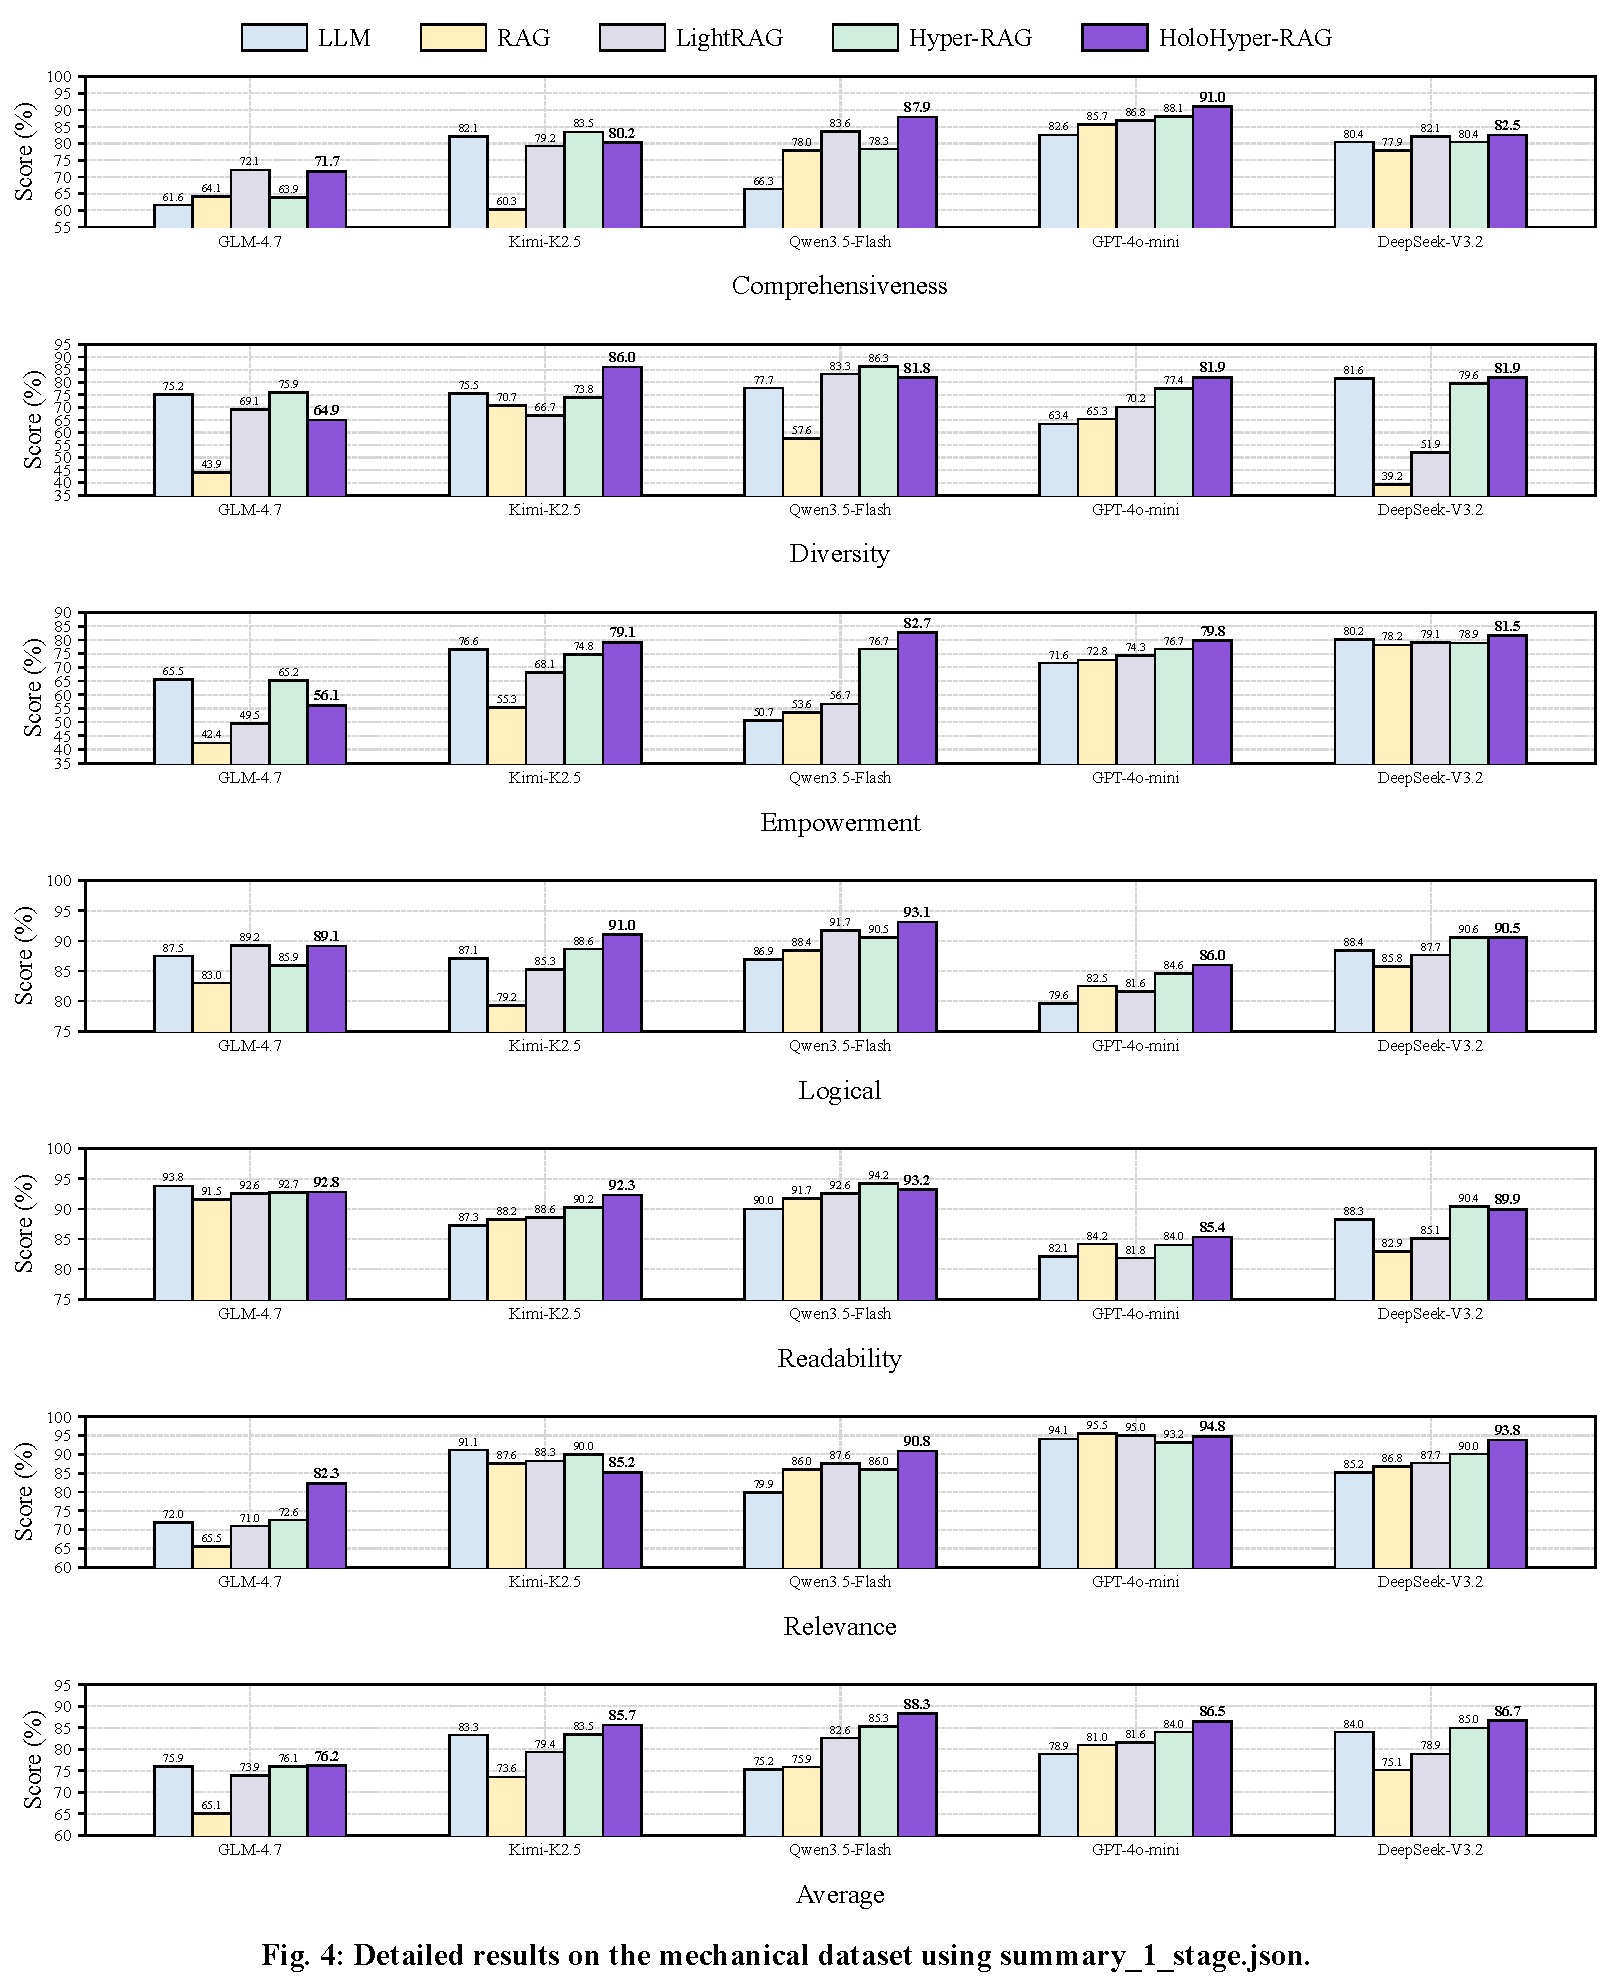
\includegraphics[width=0.95\textwidth]{figs/summary_1_stage_mechanical_grouped_bars.pdf}
\caption{Average performance of different RAG methods on the mechanical dataset under different LLM backbones.}
\label{fig:mechanical_llm_overall}
\end{figure*}

As shown in Figure~\ref{fig:mechanical_llm_overall}, performance varies across LLM backbones, indicating that answer quality depends on both retrieval quality and generation capability. HoloHyper RAG remains competitive across backbones, which suggests that its cascaded hypergraph structure provides useful evidence organization beyond a specific LLM setting.

We further evaluate the methods across the three mechanical question stages using the same LLM backbone. Figure~\ref{fig:mechanical_stage_overall} reports the average scores across different evidence depths.

\begin{figure}
\centering
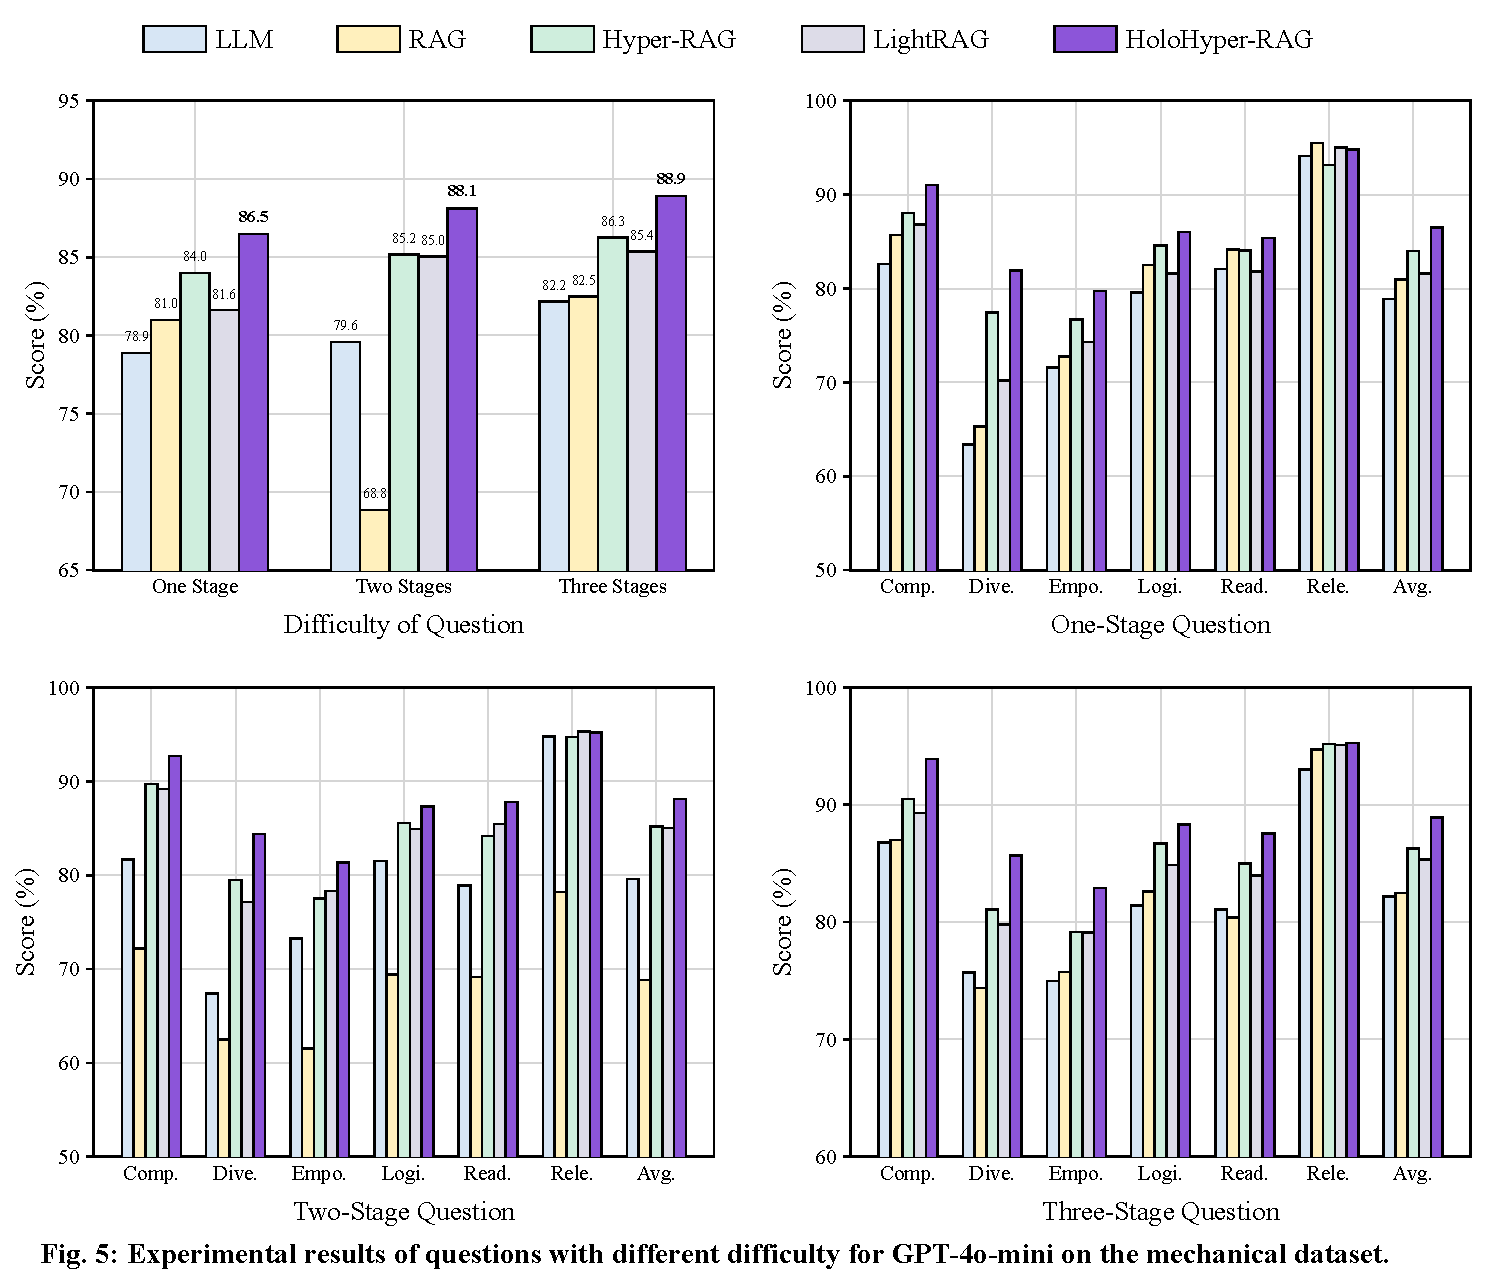
\includegraphics[width=\linewidth]{figs/gpt4o_mini_mechanical_stage_difficulty.pdf}
\caption{Average performance of different RAG methods across different question stages on the mechanical dataset.}
\label{fig:mechanical_stage_overall}
\end{figure}

As shown in Figure~\ref{fig:mechanical_stage_overall}, dense chunk retrieval is more sensitive to one-hop and two-hop questions. Graph- and hypergraph-based methods are more stable because they exploit structural associations among textual units. HoloHyper RAG further benefits from topic-guided local candidate recall, sentence-level reranking, and shared-entity topological multi-hop expansion, which together improve evidence selection under increasing evidence depth. This trend is consistent with HotpotQA and complex KBQA studies, which show that multi-hop questions often require linking supporting facts or entity-relation chains rather than retrieving a single isolated passage \citep{Yang2018HotpotQA,Lan2023ComplexKBQA}.
\subsection{Cross-domain Evaluation}
To answer RQ2, we fix the backbone LLM and compare different retrieval methods across multiple datasets. The evaluated datasets include machine-tool-related domains, such as mechanical, hydraulic, electrical, maintenance, and system, as well as general-domain datasets, including mix, pathology, and agriculture.

For each dataset, all methods use the same corpus, questions, embedding model, generation model, and evaluation protocol.

Figure~\ref{fig:cross_domain_overall} shows the average performance of different RAG methods across datasets.

\IfFileExists{figs/gpt4o_mini_dataset_method_radar.pdf}{%
\begin{figure*}[t]
\centering
\includegraphics[width=0.95\textwidth]{figs/gpt4o_mini_dataset_method_radar.pdf}%
\caption{Cross-domain performance comparison of different RAG methods under the same LLM backbone.}
\label{fig:cross_domain_overall}
\end{figure*}
}{%
\begin{figure}
\centering
\fbox{\parbox{\linewidth}{\centering Missing figure: figs/gpt4o_mini_dataset_method_radar.pdf}}
\caption{Cross-domain performance comparison of different RAG methods under the same LLM backbone.}
\label{fig:cross_domain_overall}
\end{figure}
}

As shown in Figure~\ref{fig:cross_domain_overall}, performance varies across domains because the datasets differ in terminology, document organization, entity distribution, and reasoning patterns. HoloHyper RAG remains competitive in both machine-tool and general-domain settings. This result indicates that topic-, chunk-, sentence-, and entity-level modeling helps the framework adapt to evidence with different granularities.
\subsection{Ablation Study}

To answer RQ3, we conduct a component-wise ablation study on the mechanical dataset. Each variant removes one component from HoloHyper RAG while keeping the corpus, questions, embedding model, generation model, and evaluation protocol unchanged. This protocol isolates the effect of individual retrieval modules, following the standard practice of component ablation in retrieval and graph-learning systems \citep{Velickovic2018GAT,Khattab2020ColBERT,Santhanam2022ColBERTv2}.

\begin{table*}[t]
\centering
\caption{Component-wise ablation results on the mechanical dataset. All scores are evaluated using GPT-4o-mini under the same protocol. $\Delta$ denotes the average-score change compared with the full model.}
\label{tab:ablation_results}
\setlength{\tabcolsep}{4pt}
\begin{tabular}{lcccccccc}
\hline
Ablated component & Comp. & Div. & Emp. & Log. & Read. & Rel. & Avg. & $\Delta$ \\
\hline
None (full HoloHyper RAG) & 86.60 & 71.40 & 74.24 & 84.30 & 82.50 & 91.70 & 81.79 & 0.00 \\
Local attention fusion & 83.00 & 66.70 & 72.70 & 82.50 & 80.20 & 91.40 & 79.42 & -2.37 \\
Dynamic multi-granularity scoring & 85.20 & 68.90 & 73.30 & 83.00 & 81.26 & 90.80 & 80.41 & -1.38 \\
Query-side cascaded enhancement & 85.40 & 70.20 & 73.50 & 83.10 & 82.92 & 91.90 & 81.17 & -0.62 \\
Topic-guided local candidate recall & 83.50 & 68.20 & 72.82 & 82.84 & 81.34 & 90.34 & 79.84 & -1.95 \\
Entity-level MaxSim matching & 84.00 & 65.20 & 73.34 & 82.20 & 81.80 & 91.30 & 79.64 & -2.15 \\
Shared-entity topological multi-hop expansion & 82.90 & 70.40 & 73.50 & 81.40 & 81.00 & 90.00 & 79.87 & -1.92 \\
\hline
\end{tabular}
\end{table*}

As shown in Table~\ref{tab:ablation_results}, the full HoloHyper RAG framework achieves the highest average score. Removing local attention fusion causes the largest decrease, reducing the average score from 81.79 to 79.42. This result shows that topology-aware representation fusion is important for injecting contextual information into chunk, sentence, and entity representations.

Entity-level MaxSim matching and topic-guided local candidate recall also produce clear performance drops, with average-score decreases of 2.15 and 1.95 points, respectively. The entity-level variant shows the largest reduction in Diversity, indicating that context-enhanced entity anchors help retrieve fine-grained technical evidence. This observation is consistent with late-interaction retrieval and entity-aware representation studies, where fine-grained token or entity alignment provides stronger matching signals than a single compressed vector. The topic-routing variant confirms that topic-guided local candidate recall provides an effective candidate scope before sentence-level reranking.

Shared-entity topological multi-hop expansion decreases the average score by 1.92 points, which confirms its role in recovering evidence distributed across textual units. Dynamic multi-granularity scoring produces a 1.38-point drop, showing that adaptive score fusion is more effective than fixed chunk-, sentence-, and entity-level weighting. Query-side cascaded enhancement has the smallest decrease in this first-stage setting. Overall, the ablation results support the combined use of topology-aware representation fusion, adaptive multi-granularity scoring, entity-level matching, and shared-entity multi-hop retrieval.
\subsection{Retrieval Efficiency Analysis}

To answer RQ4, we measured retrieval efficiency on all 50 first-stage questions in the Mechanical dataset. For each retrieval-based method, the online retrieval time was averaged over the 50 questions and paired with the corresponding average answer-quality score. The reported retrieval time includes online retrieval and context construction only. Offline index construction, final answer generation, and LLM-as-a-judge evaluation are not included. Separating online retrieval latency from offline indexing and generation cost follows the evaluation logic of efficient dense and late-interaction retrieval studies \citep{Karpukhin2020DPR,Khattab2020ColBERT,Santhanam2022ColBERTv2}.

\begin{figure}
\centering
\includegraphics[width=\linewidth]{figs/retrieval_efficiency_mechanical_q1.pdf}
\caption{Average retrieval efficiency on 50 first-stage mechanical questions. Each point reports the average retrieval time and the corresponding average answer-quality score of a retrieval method.}
\label{fig:retrieval_efficiency}
\end{figure}

As shown in Figure~\ref{fig:retrieval_efficiency}, SimpleRAG has the lowest retrieval latency because it performs direct dense matching over text chunks. LightRAG also remains relatively efficient, while HyperRAG and HoloHyper RAG require more retrieval time because they perform structured retrieval over graph or hypergraph representations.

The efficiency result should be interpreted together with answer quality. HoloHyper RAG achieves the highest average score while keeping retrieval time comparable to the HyperRAG baseline. This indicates that the additional topic-guided recall, sentence-level reranking, entity matching, and shared-entity multi-hop expansion introduce structured retrieval cost, but they also improve evidence organization for knowledge-intensive mechanical questions.

\subsection{Discussion}

The results indicate that HoloHyper RAG is most effective when evidence is distributed across multiple semantic granularities. In machine-tool documents, topic-level context, component-level facts, sentence-level constraints, and entity-level relations are often interdependent. The cascaded multi-granularity hypergraph helps preserve these dependencies, while topic-guided recall, sentence reranking, entity-level MaxSim matching, and shared-entity multi-hop expansion jointly reduce coarse semantic drift and improve fine-grained evidence selection.

The ablation results further show that the performance gain is not produced by a single component. Removing local attention fusion causes the largest average-score decrease, which suggests that topology-aware contextual fusion is important for building useful chunk, sentence, and entity representations. The drops caused by removing entity-level MaxSim matching, topic-guided local candidate recall, and shared-entity topological multi-hop expansion also support the need to combine macro-level candidate pruning with micro-level factual matching. The relatively small decrease from removing query-side cascaded enhancement may be related to the first-stage setting, where many questions are direct factual queries.

The framework also has clear boundaries. Its benefit is likely to be stronger in corpora with repeated entities, hierarchical descriptions, and cross-sentence dependencies than in weakly structured texts. It also introduces more retrieval cost than flat dense retrieval, although the measured latency remains comparable to the HyperRAG baseline. In addition, errors in chunking, topic clustering, or entity extraction can propagate through the cascaded hypergraph, and shared-entity expansion may retrieve noisy evidence when frequent entities create weak logical links. Future work should therefore focus on entity normalization, adaptive multi-hop stopping, and human-verified evaluation on larger and more diverse datasets.

% To print the credit authorship contribution details
\printcredits

%% Loading bibliography style file
%\bibliographystyle{model1-num-names}
\bibliographystyle{elsarticle-num-names}

% Loading bibliography database
\bibliography{cas-refs}

% Biography
%\bio{}
% Here goes the biography details.
%\endbio

%\bio{pic1}
% Here goes the biography details.
%\endbio

\end{document}



